\section{Results and Analysis}
\label{sec:results-analysis}

% \textcolor{red}{This section should present the obtained results and provide an insightful analysis of them. You can present the results using graphs, tables, or any other visualization method suits your purpose. Do not forget to include proper captions \cite{zobel2014graphs} in any of these illustration methods you use. You do not need to provide any execution details as they are already presented in Sec.~\ref{sec:experimentation}.}

% \textcolor{red}{A good practise would be to compare your algorithm with a simpler approach, such as (a) a naive method, (b) a Hill Climbing approach, or (c) a simple evolutionary algorithm. In the third case, you can use the simpler version of the algorithm you developed, i.e., the original algorithm without your modifications. In that case, you should briefly describe the comparing method(s) in Sec.~\ref{sec:experimentation}. Alternatively, you can use some reference results derived from the repositories you found some benchmark instances.}

% \textcolor{red}{To display tables, the \texttt{booktabs} package might be useful. For example, Table~\ref{tab:results_example} shows how you should increase the  size of $n$, when running your code. You can advice \cite{zobel2014graphs} to see a few examples of proper tables.}

\subsection{Bayesian optimization results}

We Bayesian optimization to find the optimal population size and mutation rate for the GA. The results are shown in Figure~\ref{fig:bayesian_optimization_results}.

\subsubsection{Optimization progress}

From the first chart, the difference between the best score and the worst score is small. It means that the GA is stable and the hyperparameters are good.

\subsubsection{Population size vs Performance}

From the second chart, we can see population size around 100 and 900 can find the solution in a short time, while score is more discreted at 900 population size. Thus the average time of solving puzzle at 900 population size is costlier than 150 population size.

\subsubsection{Mutation rate vs Performance}

From the third chart, we can see muation rate between 0.05 and 0.15 have many times not find the solution, however the score of failer cases become lower and no solution events happened less frequently when mutation rate pass 0.20.

\subsubsection{Parameter space exploration}

From the fourth chart, the best population size is 142 and the best mutation rate is 0.230. This result is based on the best score shows in first chart.

\begin{figure}[H]
\centering
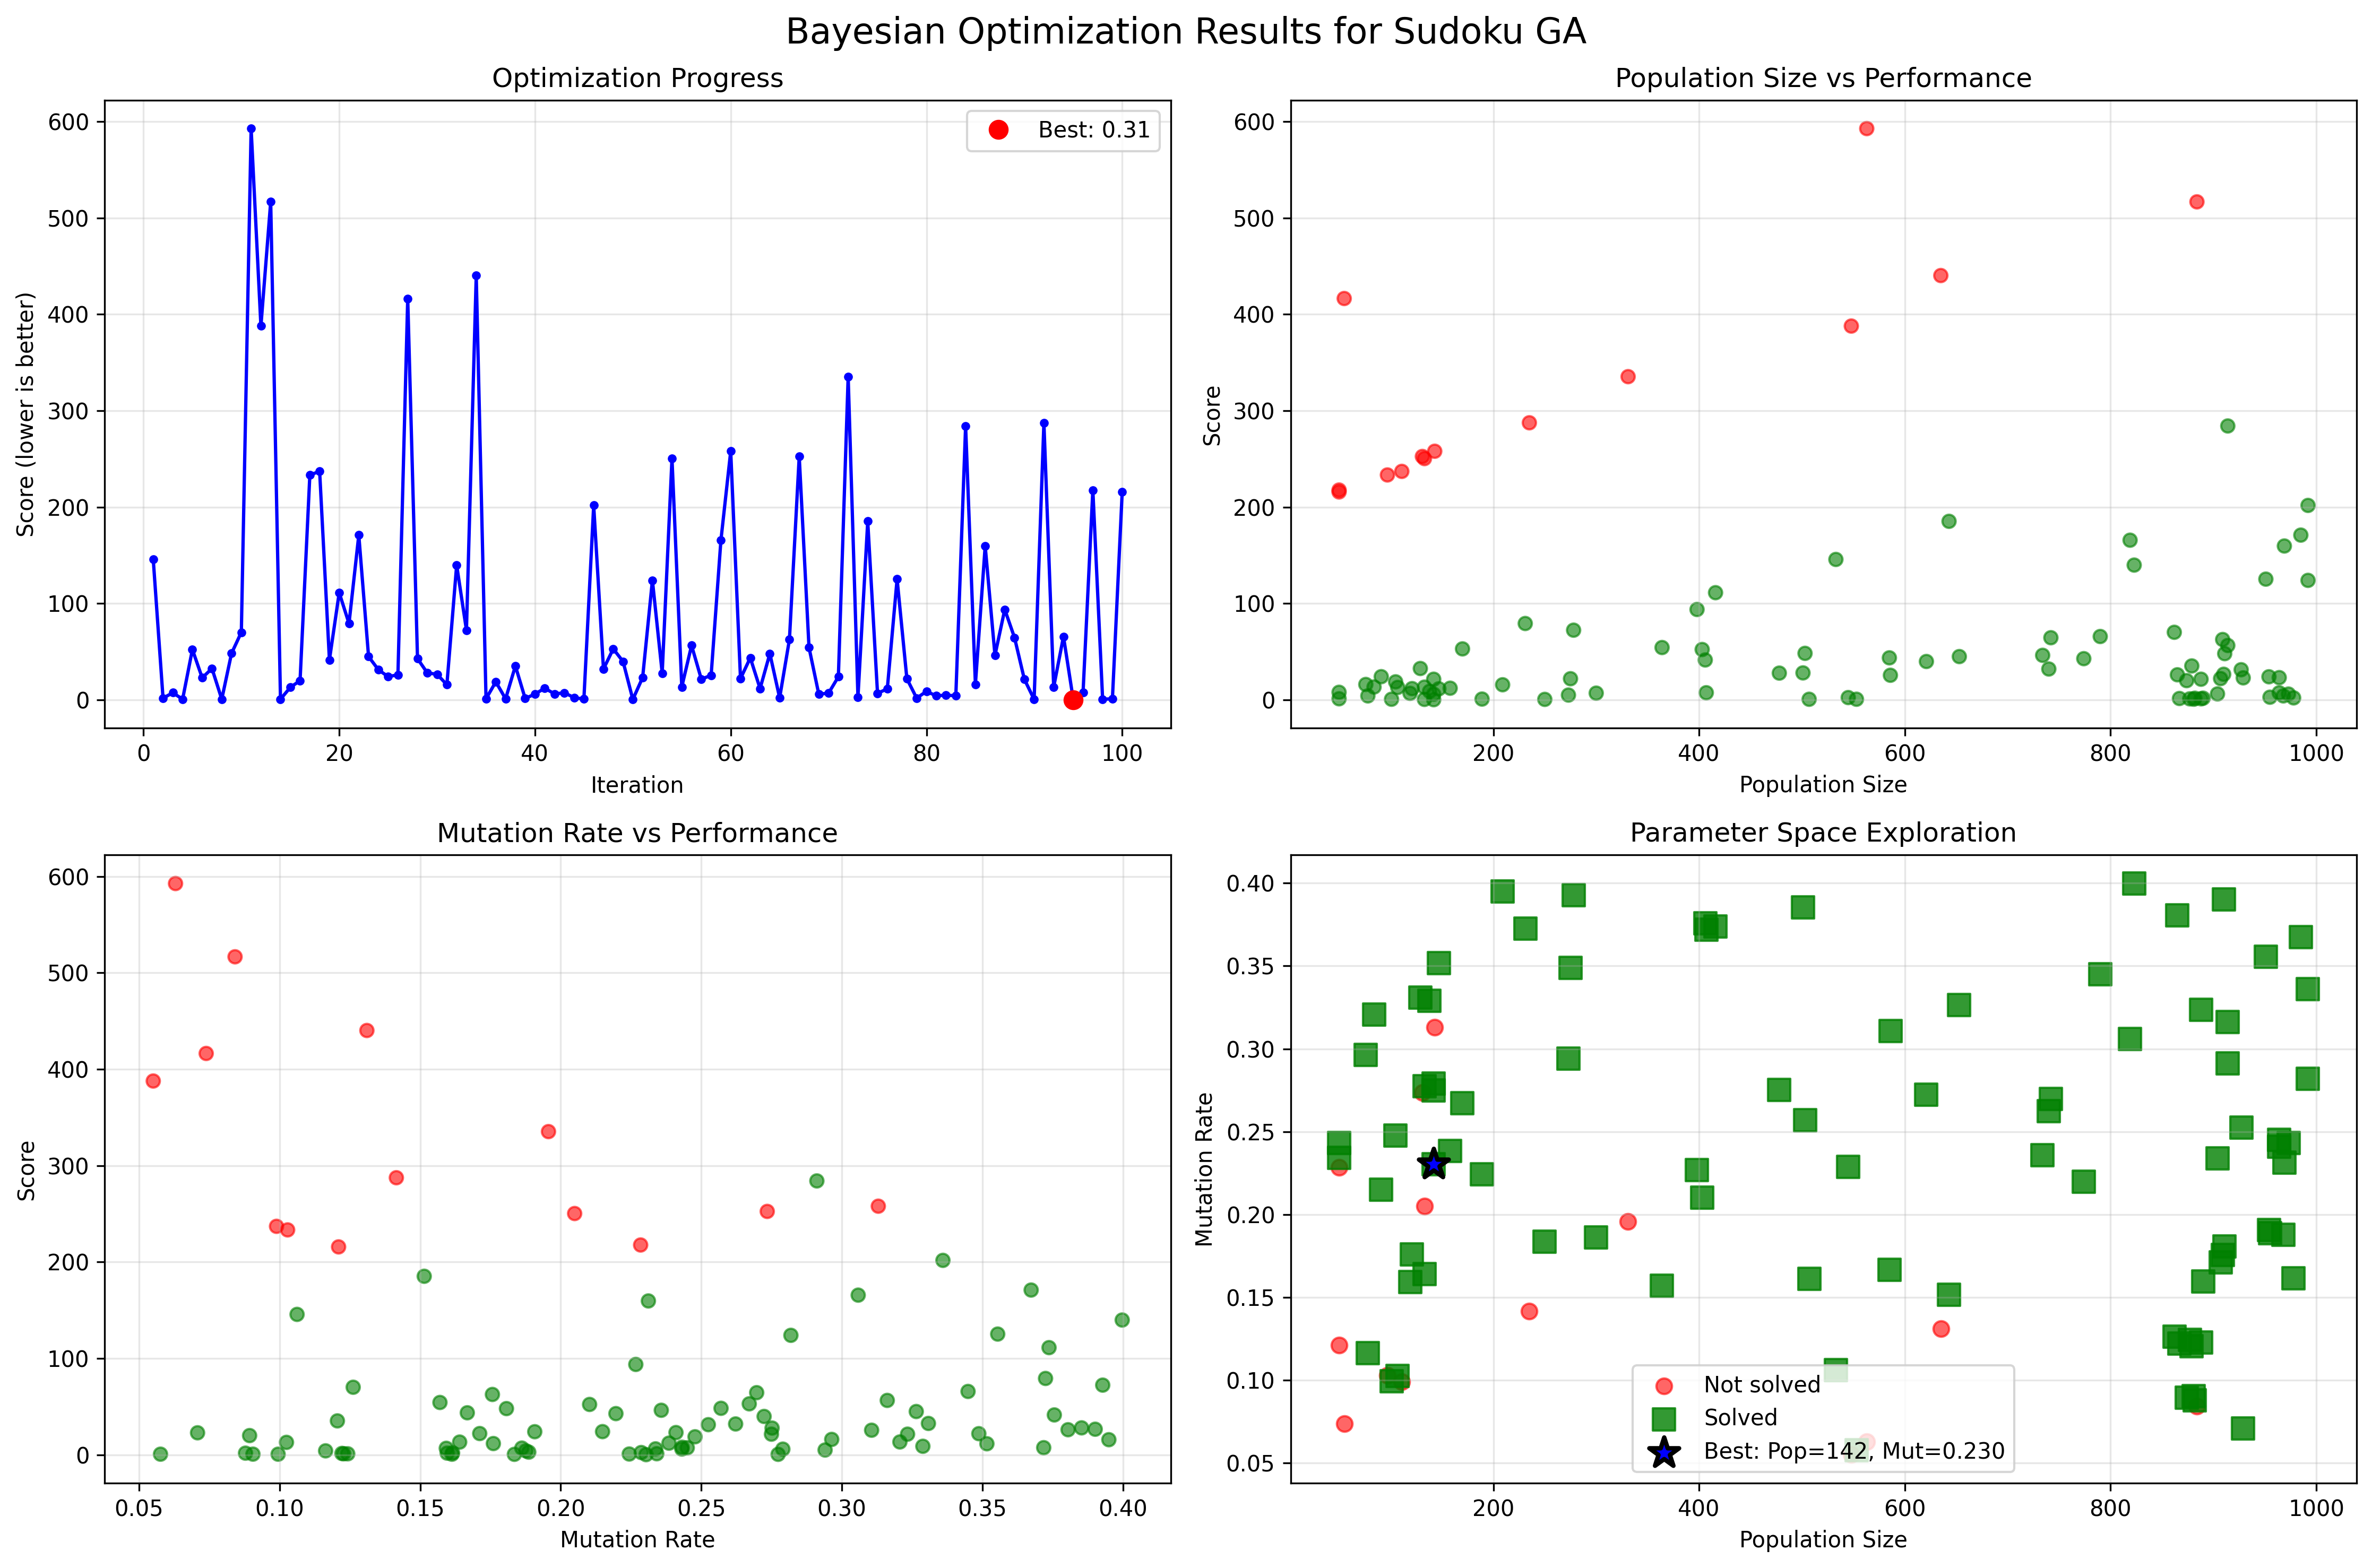
\includegraphics[width=0.8\textwidth]{resources/bayesian_optimization_results.png}
\caption{Bayesian optimization results.}
\label{fig:bayesian_optimization_results}
\end{figure}

\subsection{Test the performance of the GA with varied difficulty}

We test easy, medium and hard difficulty in same setting, and it's costly to test 1000 times for each difficulty. Thus we only test easy difficulty for 1000 times, medium one for around 400 times, and hard one for 100 times.

\subsubsection{Easy difficulty}

The charts below shows the performance of the GA with easy difficulty. There are more than 500 times find solution in less than 0.5 seconds. only around $1/20$ solutions were reached very slow which is more than 20s.
Additionly, the average execution time is 5s-ish, which is a good performance. Moreover, the execution time and generation have linear relationship. It means that if algorithm need more generations to get the solution, the more execution time it will cost.

\begin{figure}[H]
\centering
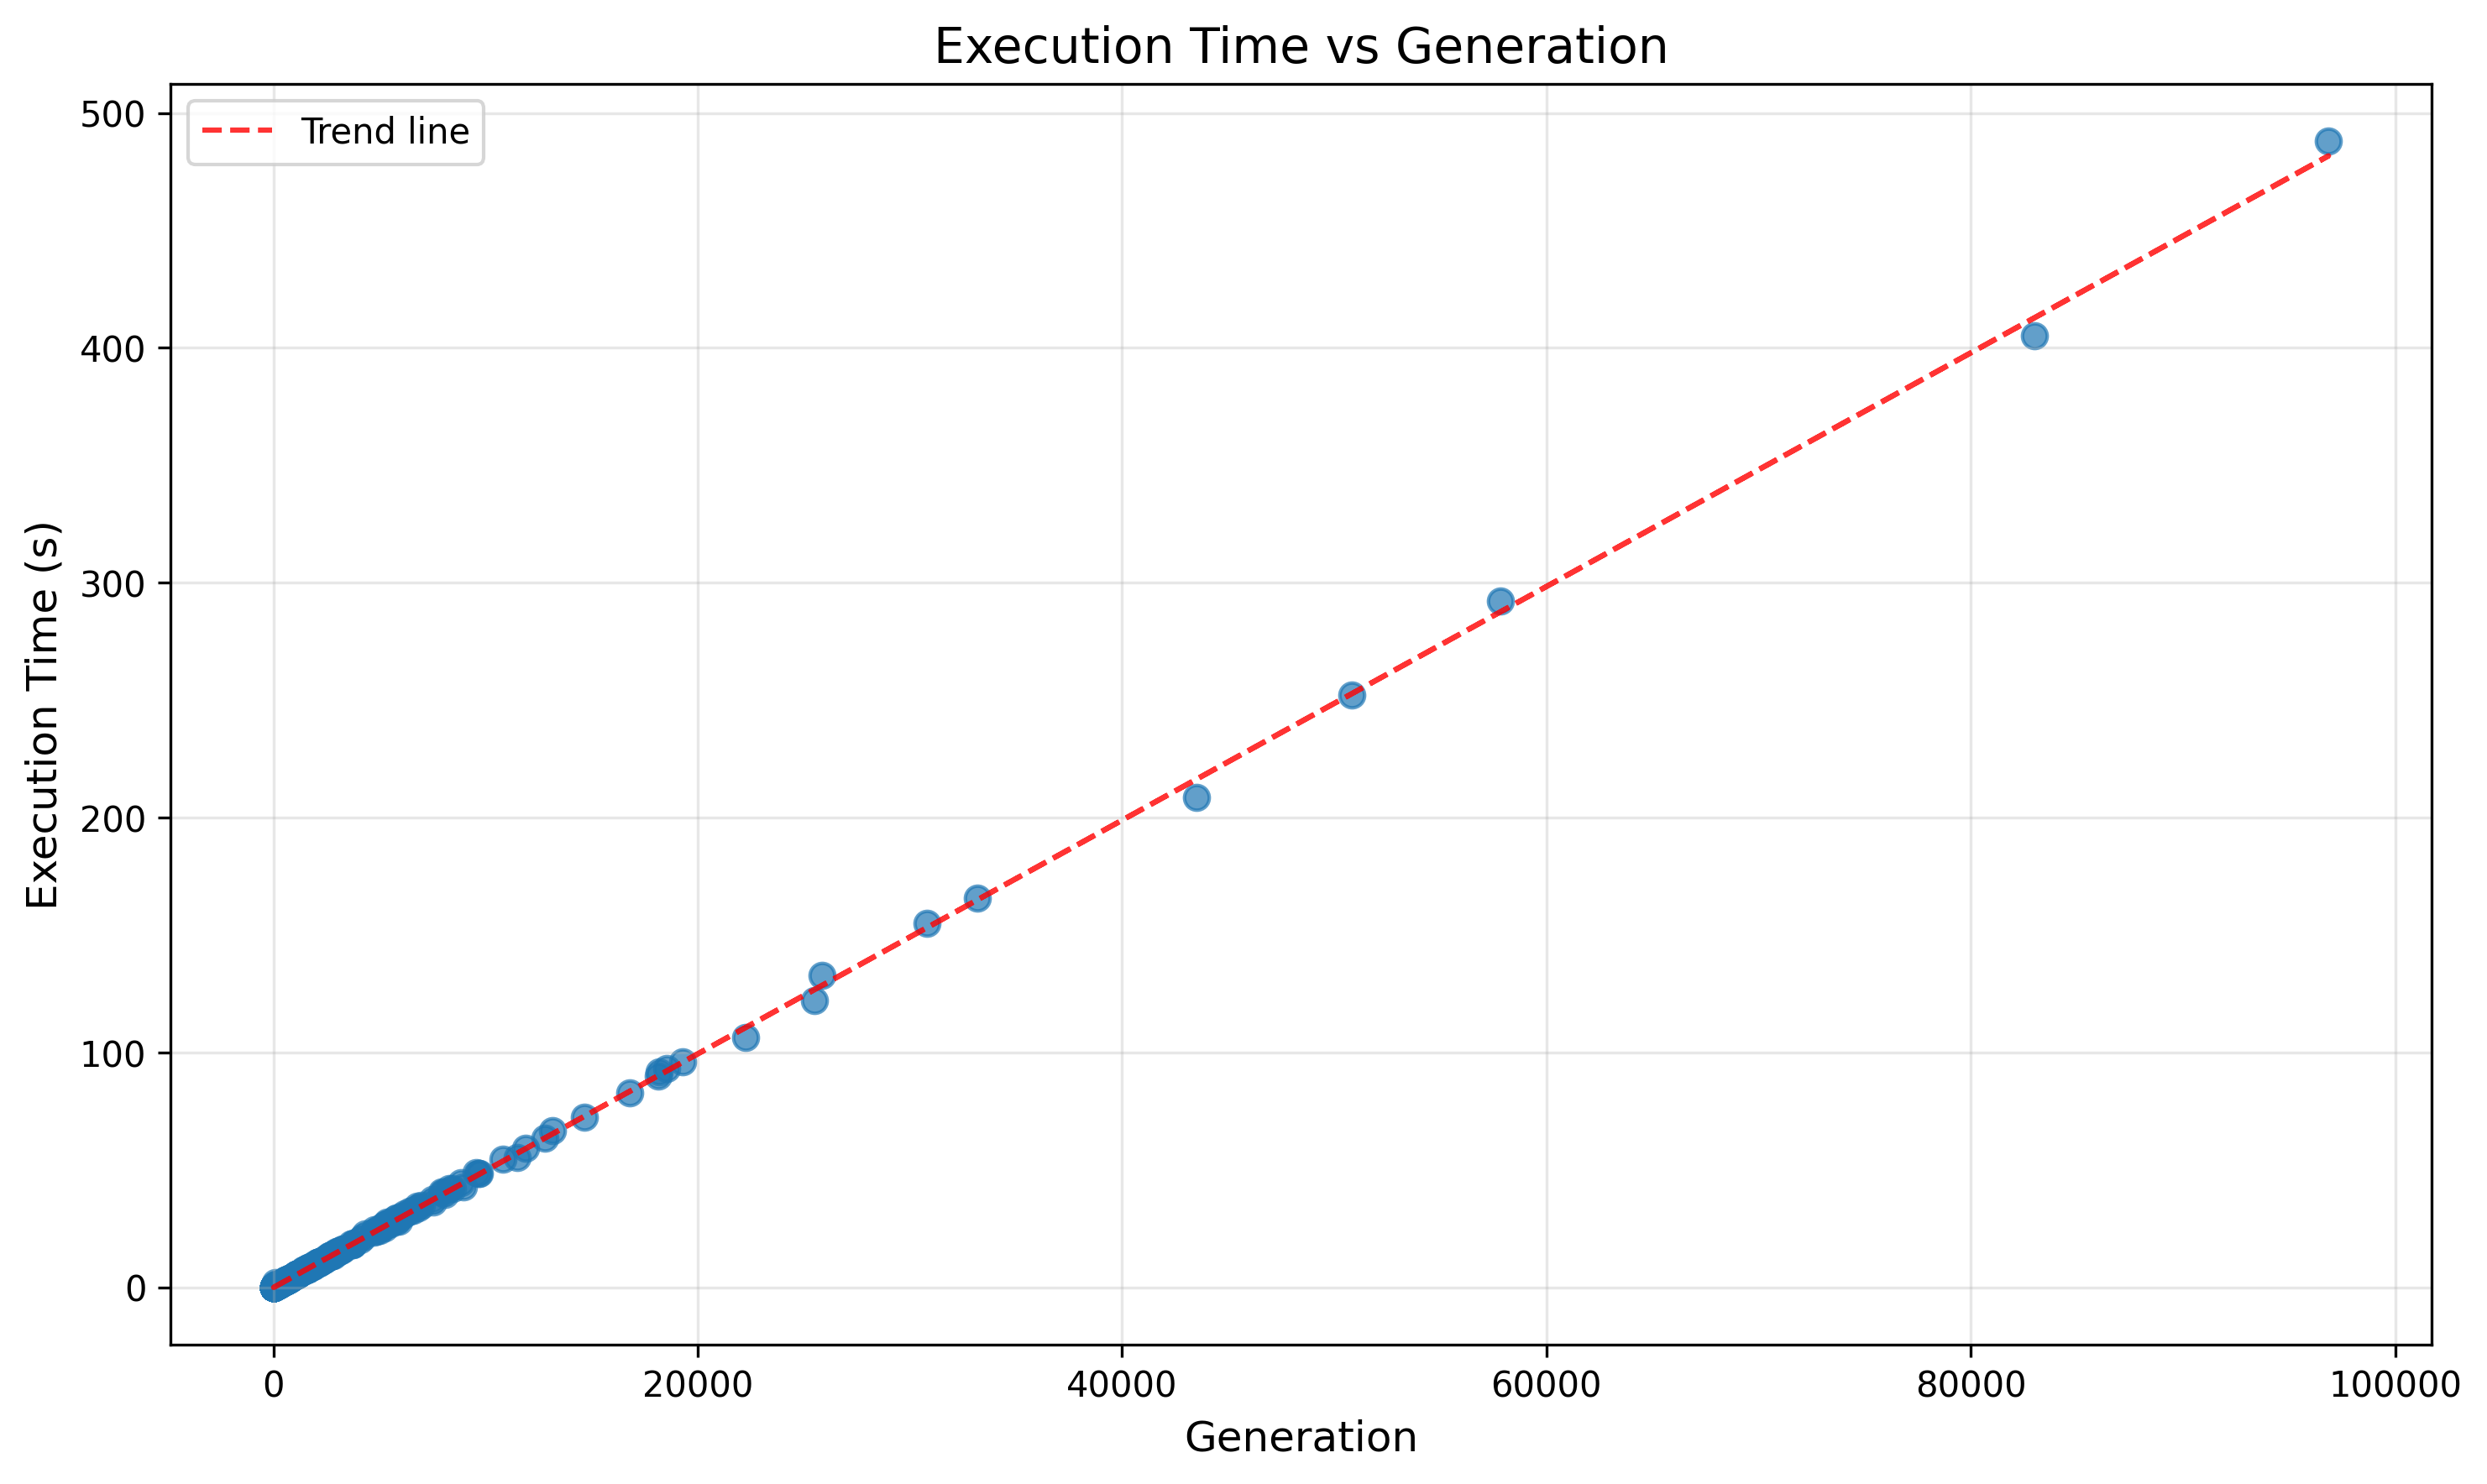
\includegraphics[width=0.8\textwidth]{resources/generation_vs_execution_time_easy.png}
\caption{Generation vs execution time for easy difficulty puzzles.}
\label{fig:generation_vs_execution_time_easy}
\end{figure}

\begin{figure}[H]
\centering
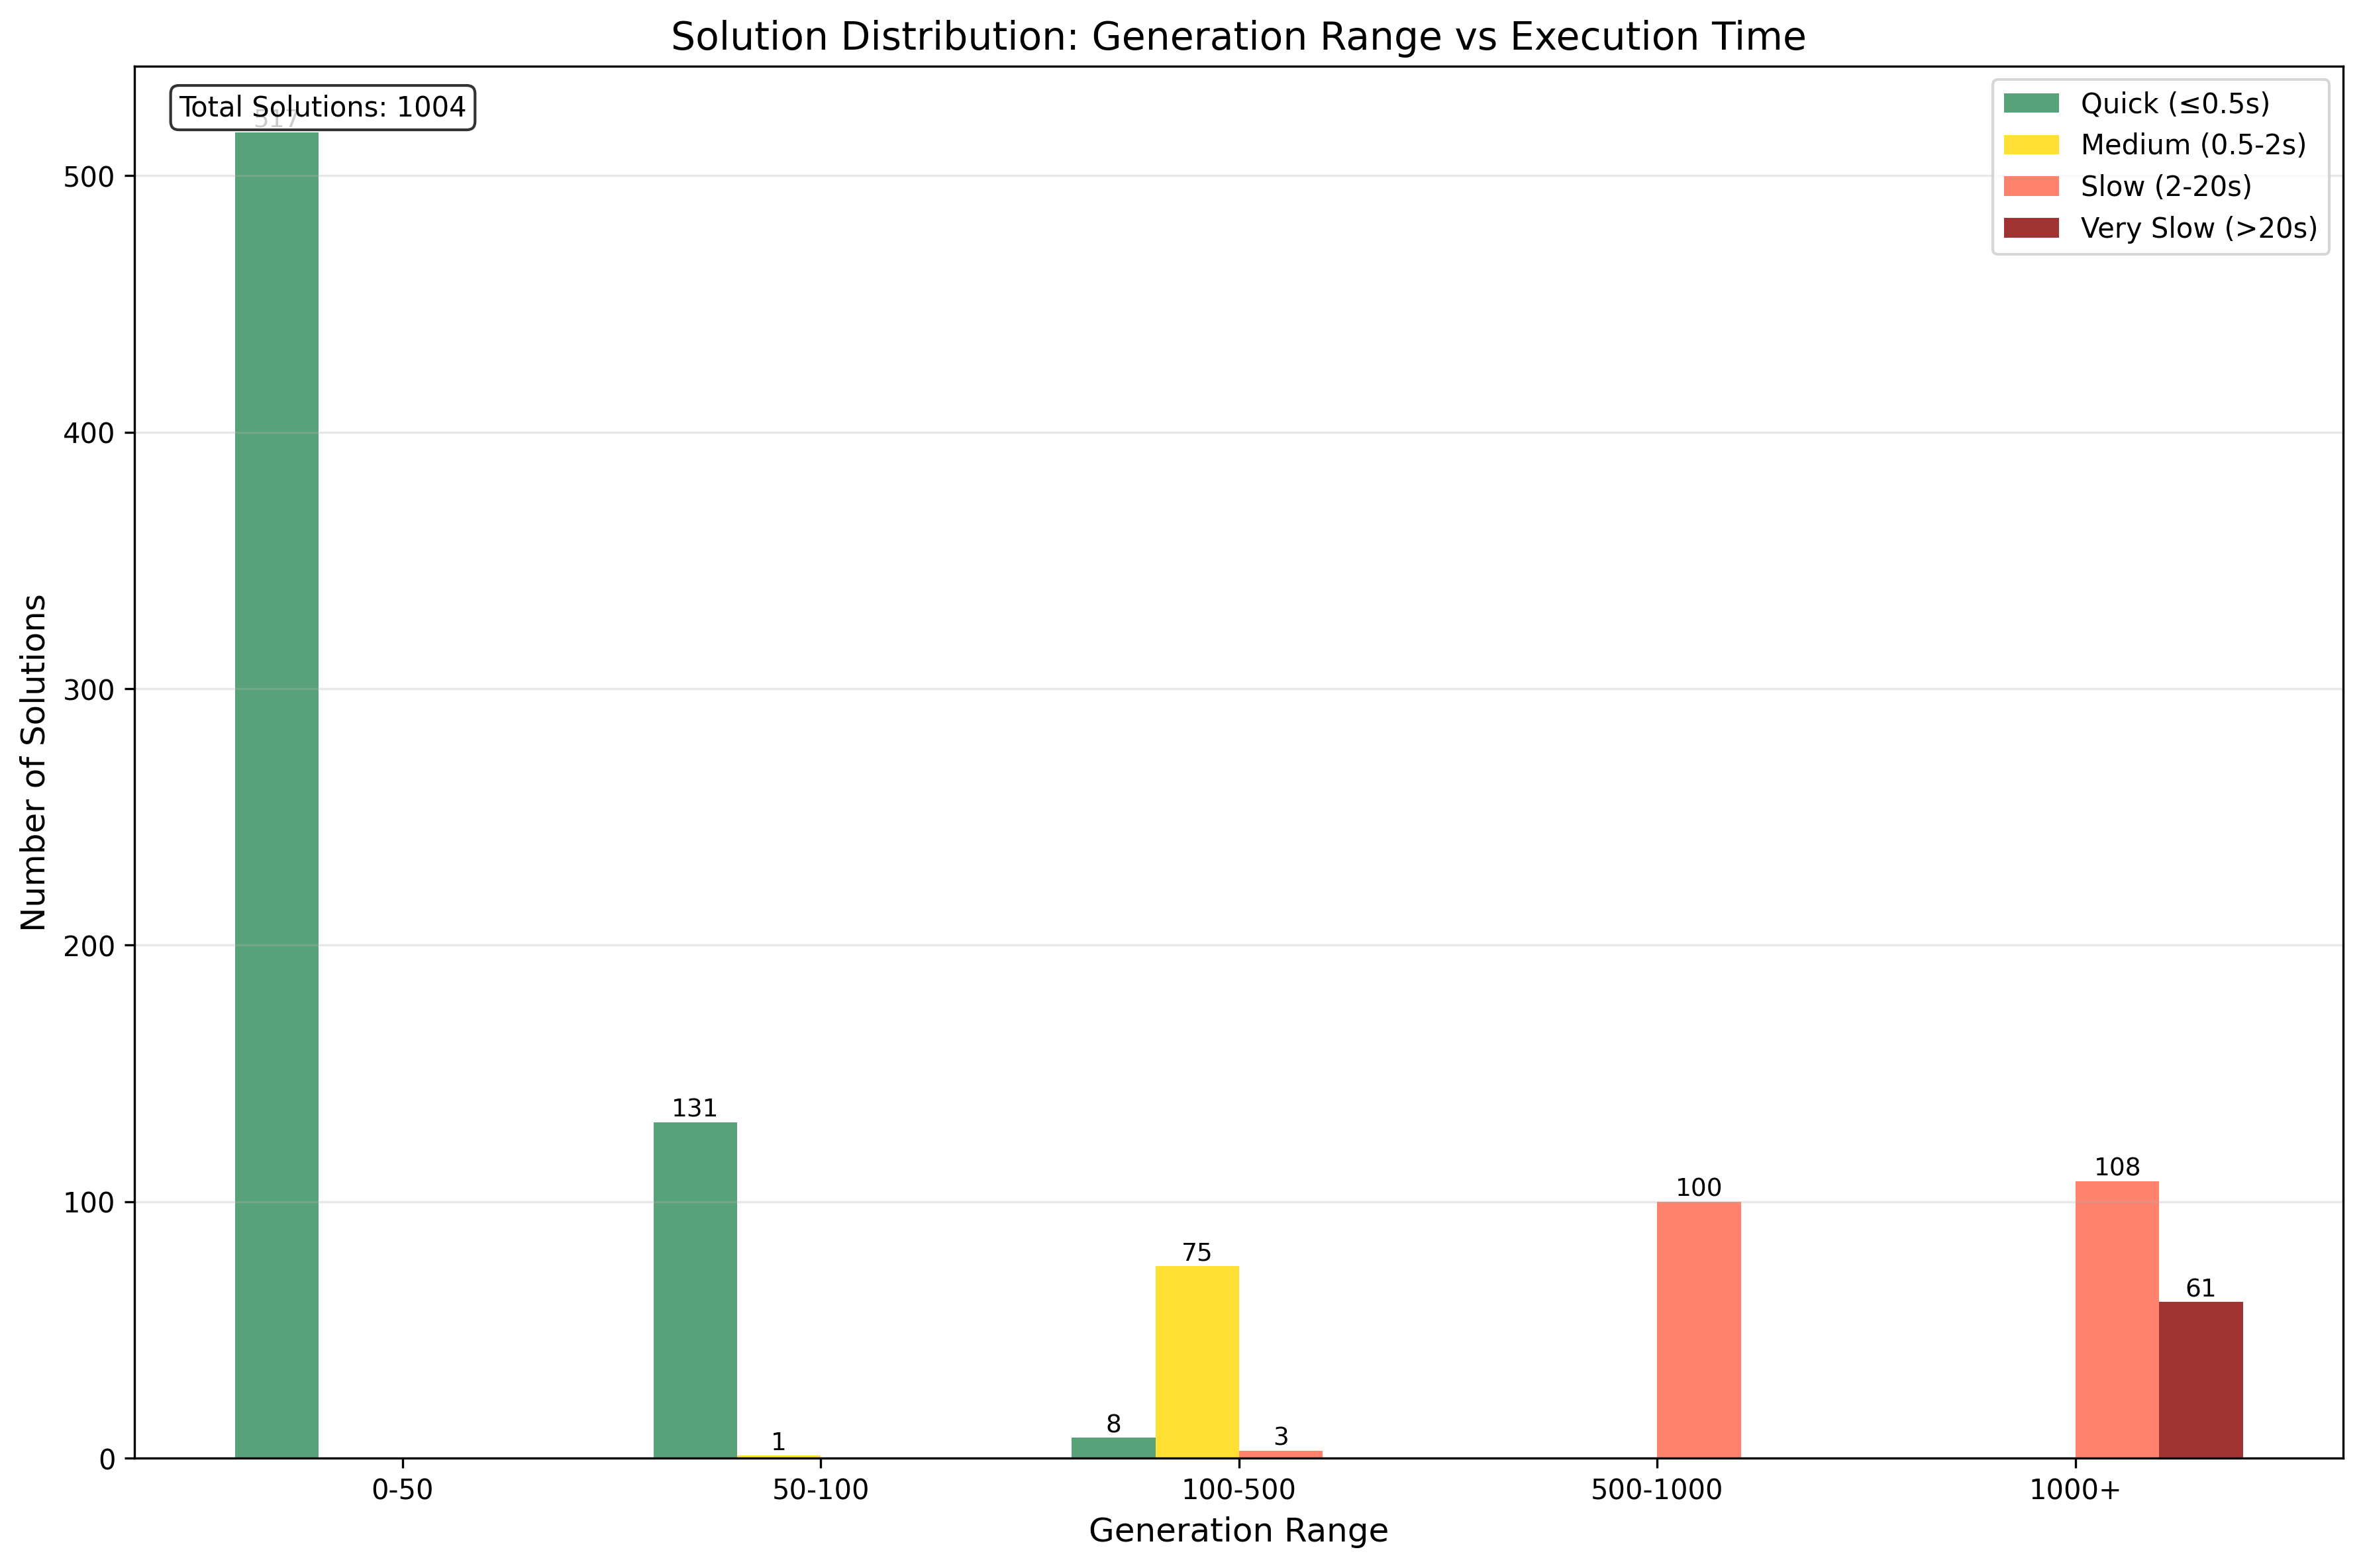
\includegraphics[width=0.8\textwidth]{resources/generation_execution_time_bars_easy.png}
\caption{Generation and execution time distribution for easy difficulty puzzles.}
\label{fig:generation_execution_time_bars_easy}
\end{figure}

\subsubsection{Medium difficulty}

The charts below shows the performance of the GA with medium difficulty, the time cost of founding solution at quick and medium time only play a small role in total cases.
However, the proportion of the getting solution in very slow is $60\%$, which is much higher comparing with easy difficulty.
Meanwhile, the execution time and generation still remain a linear relationship.

\begin{figure}[H]
\centering
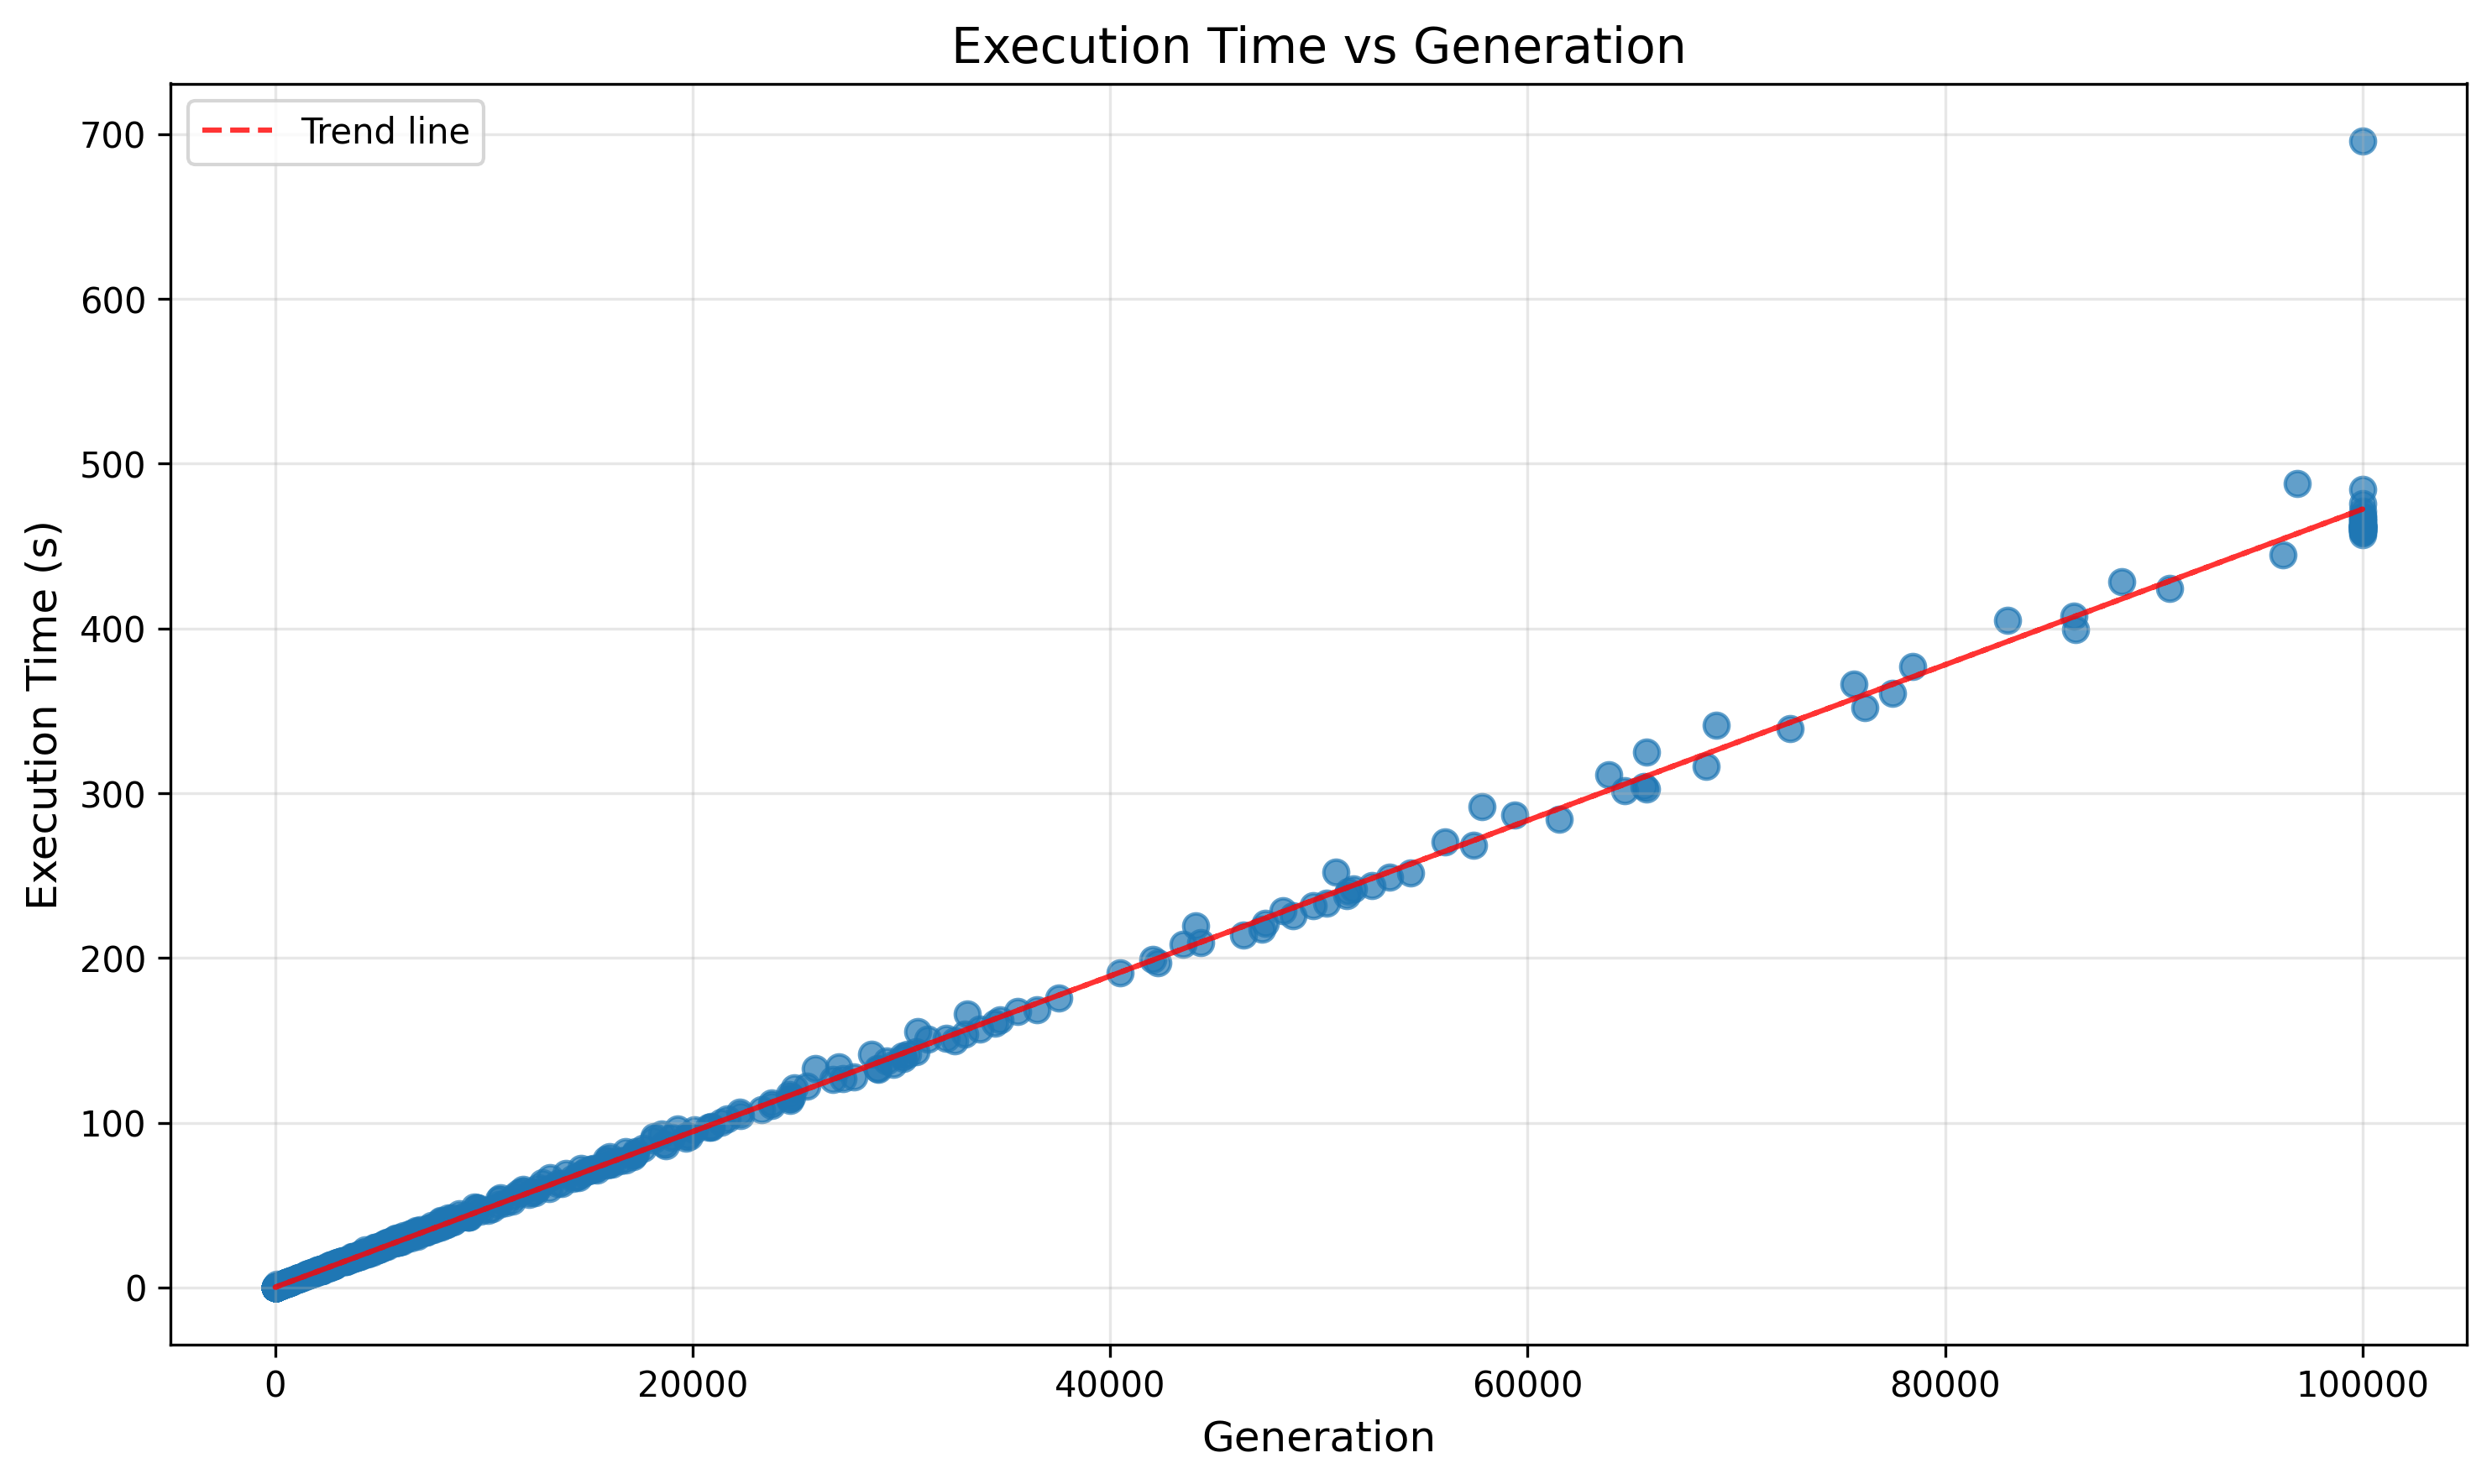
\includegraphics[width=0.8\textwidth]{resources/generation_vs_execution_time_medium.png}
\caption{Generation vs execution time for medium difficulty puzzles.}
\label{fig:generation_vs_execution_time_medium}
\end{figure}

\begin{figure}[H]
\centering
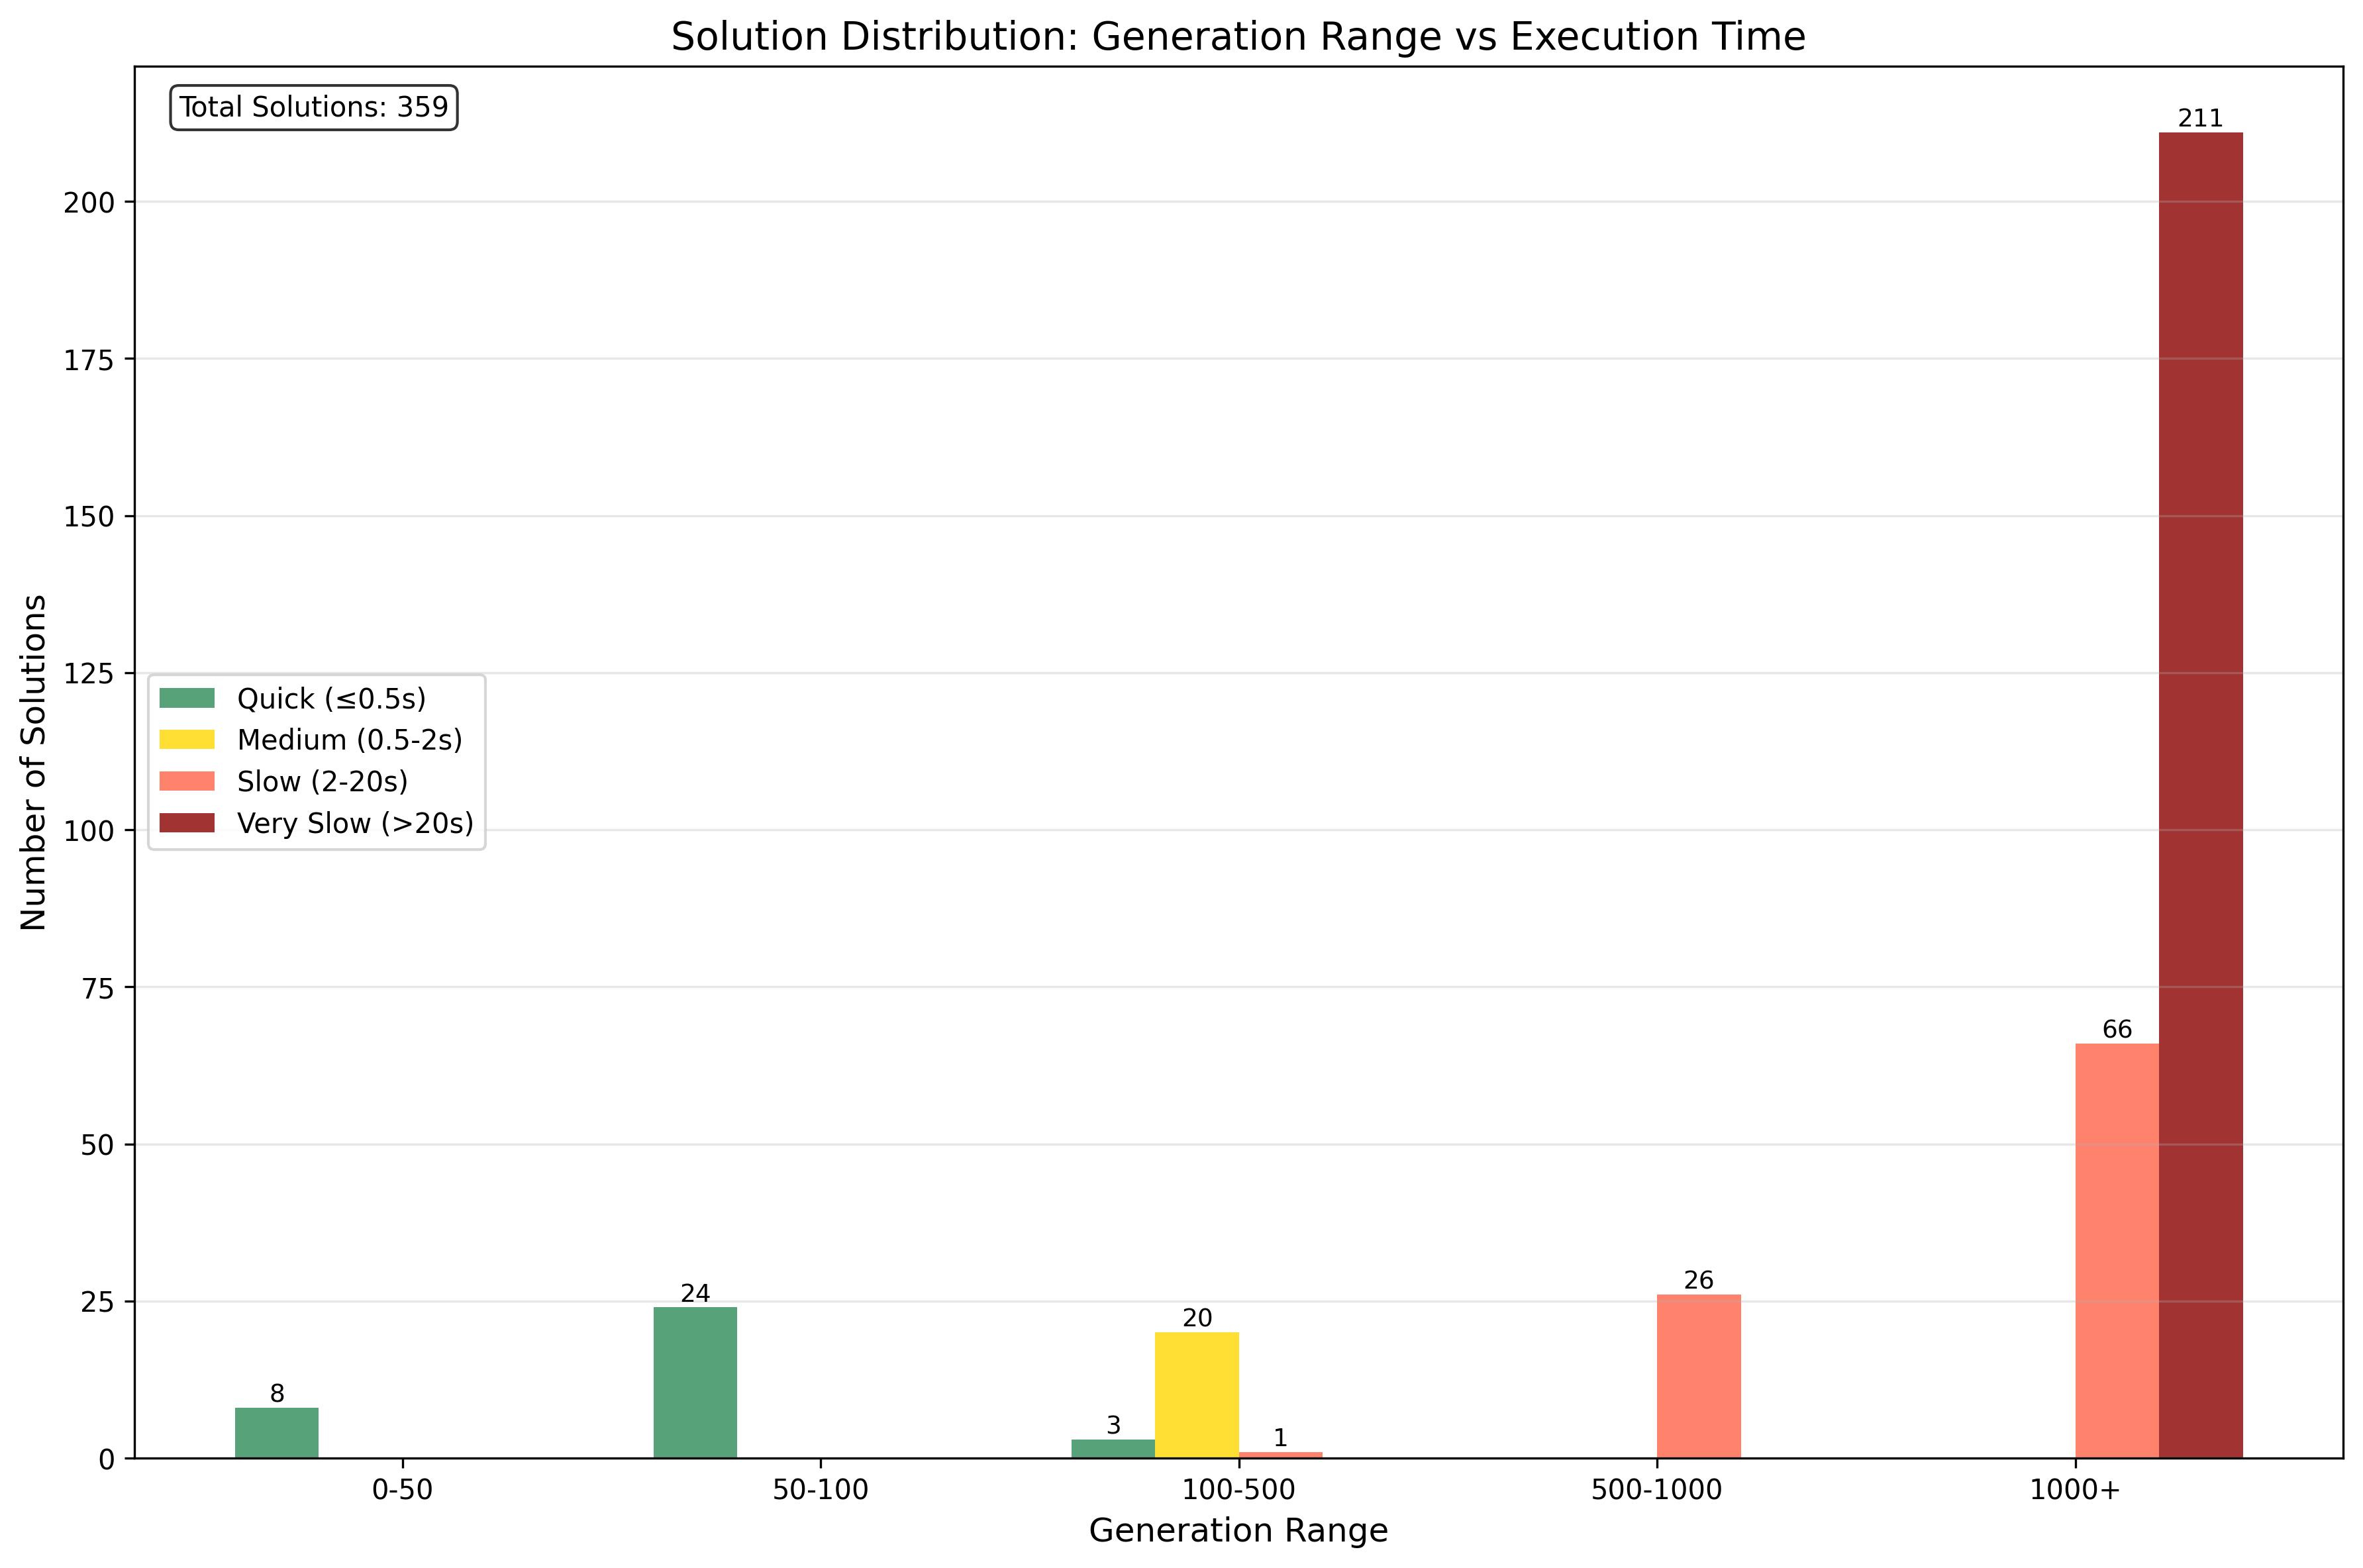
\includegraphics[width=0.8\textwidth]{resources/generation_execution_time_bars_medium.png}
\caption{Generation and execution time distribution for medium difficulty puzzles.}
\label{fig:generation_execution_time_bars_medium}
\end{figure}

\subsubsection{Hard difficulty}

The charts below shows the performance of the GA with hard difficulty, the proportion of the getting solution in very slow is $97\%$, which is much higher comparing with easy and medium difficulty.
Meanwhile, the execution time and generation still remain a linear relationship.

\begin{figure}[H]
\centering
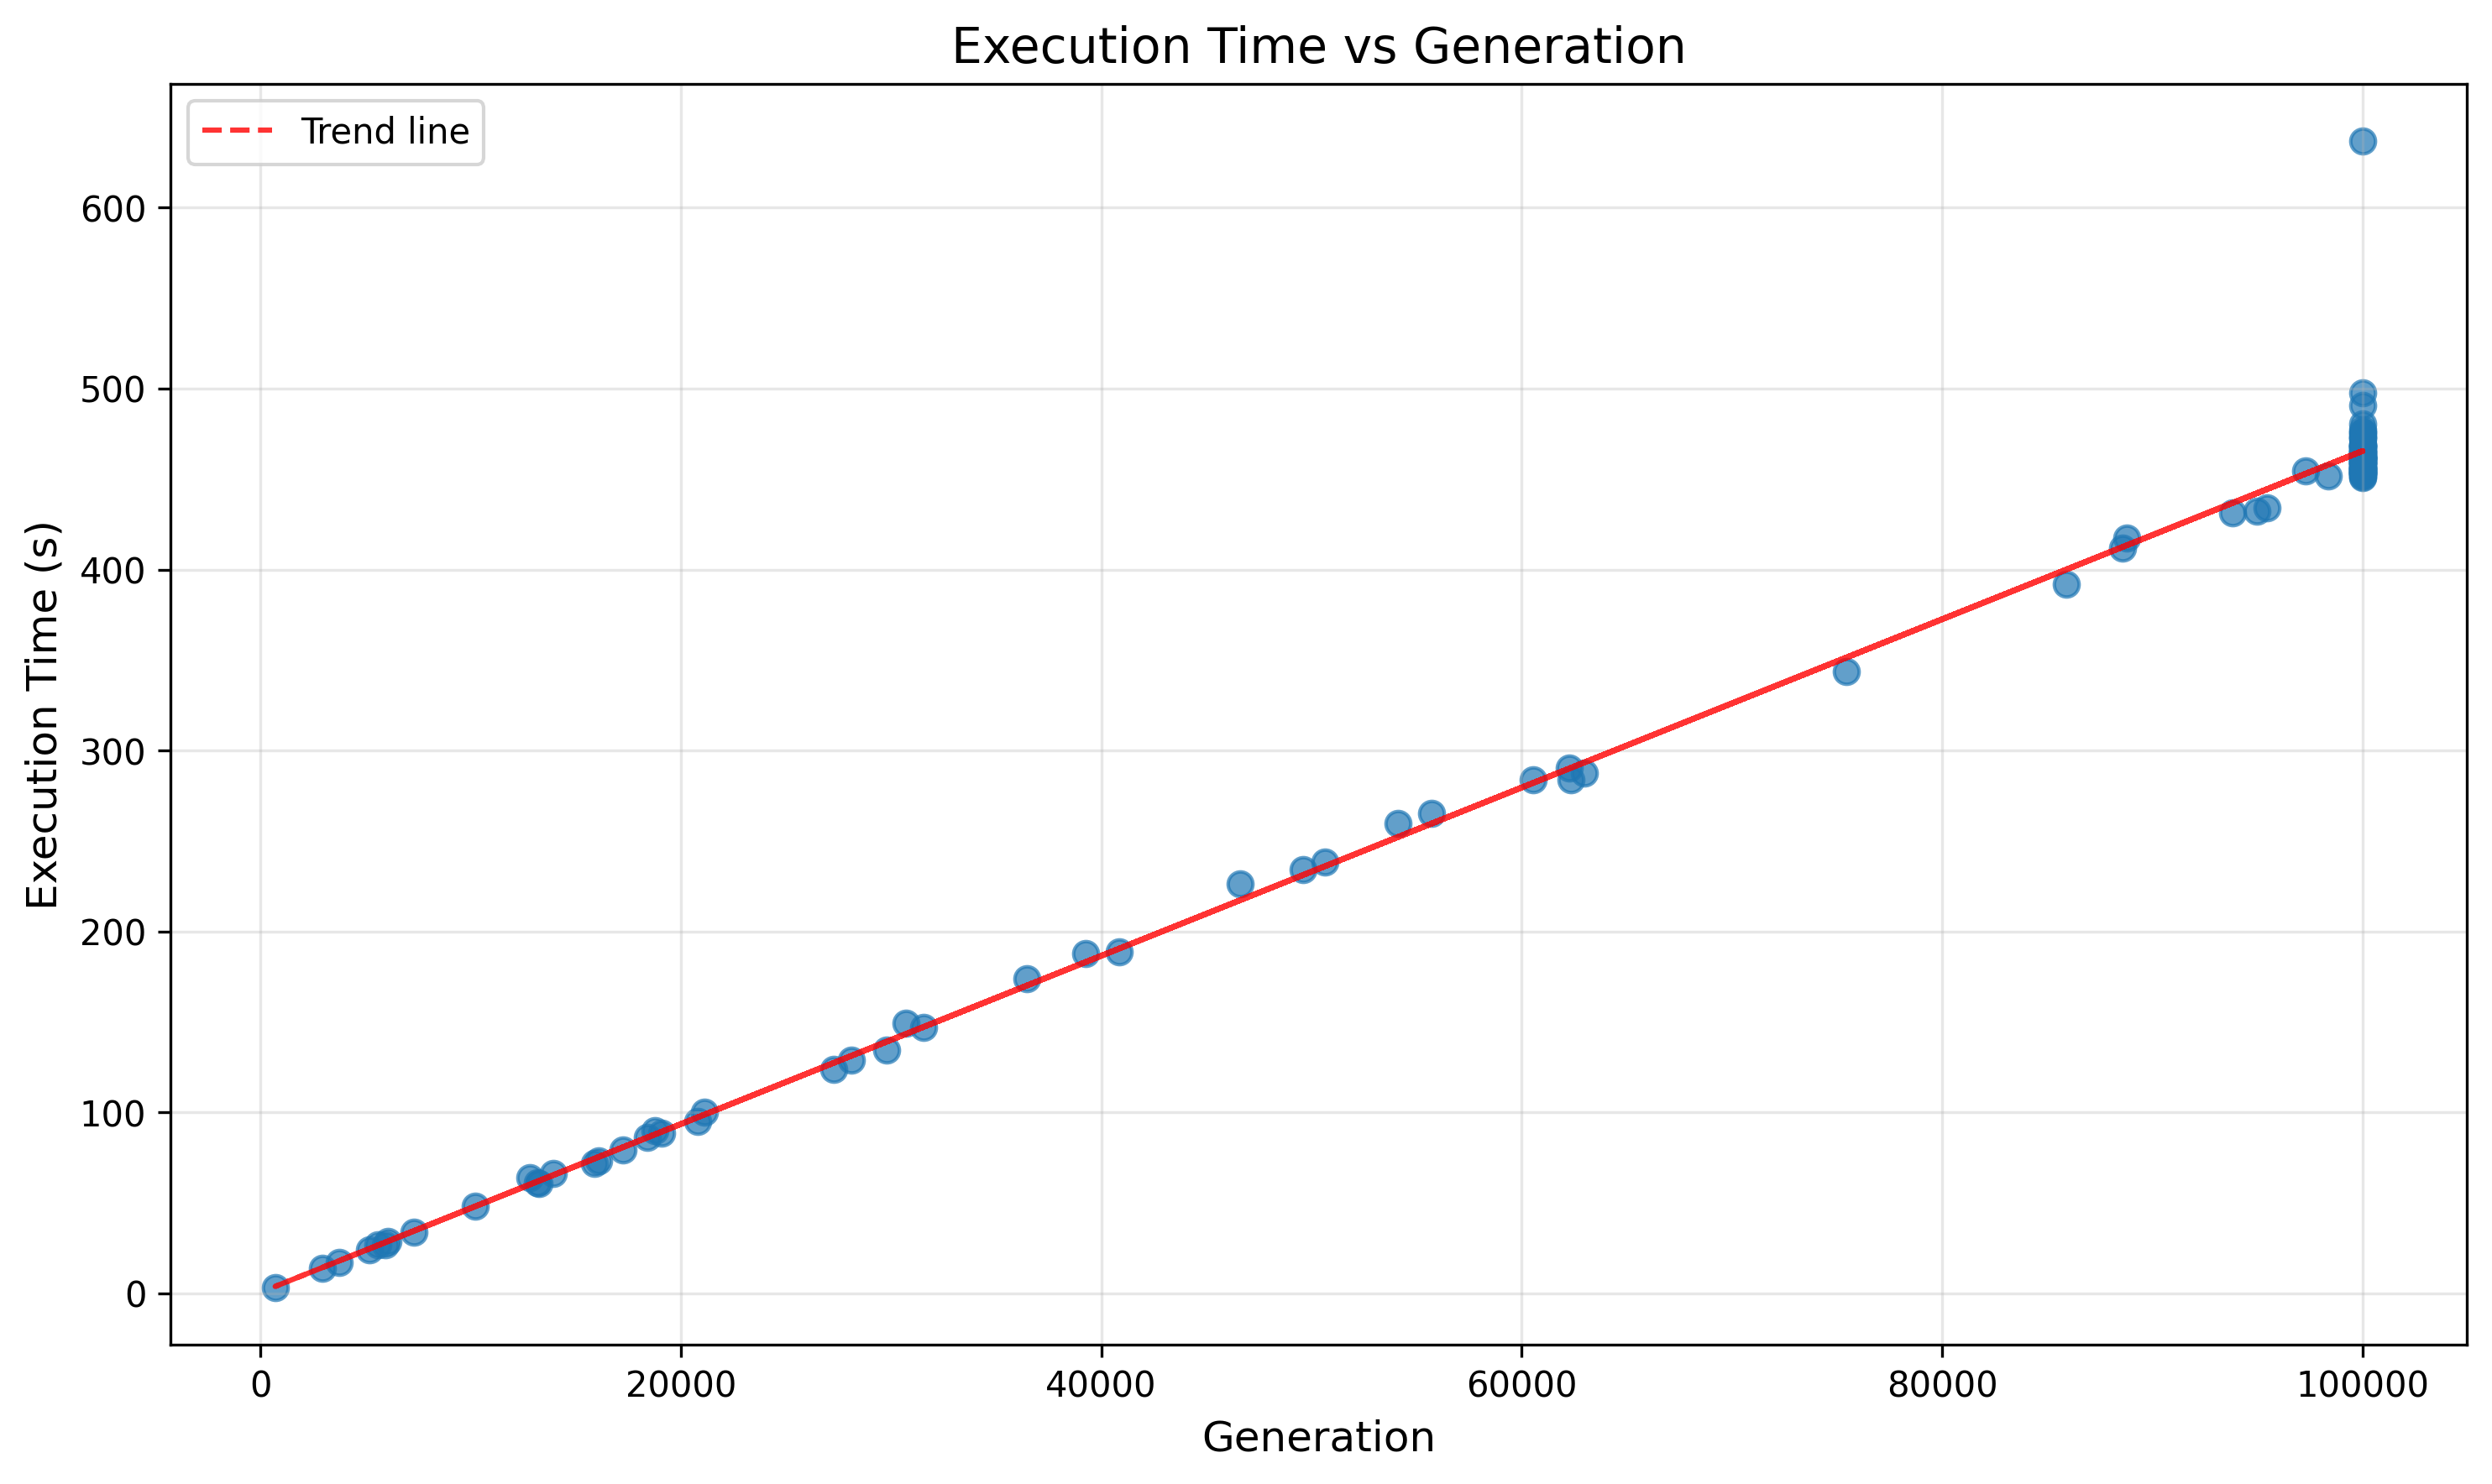
\includegraphics[width=0.8\textwidth]{resources/generation_vs_execution_time_hard.png}
\caption{Generation vs execution time for hard difficulty puzzles.}
\label{fig:generation_vs_execution_time_hard}
\end{figure}

\begin{figure}[H]
\centering
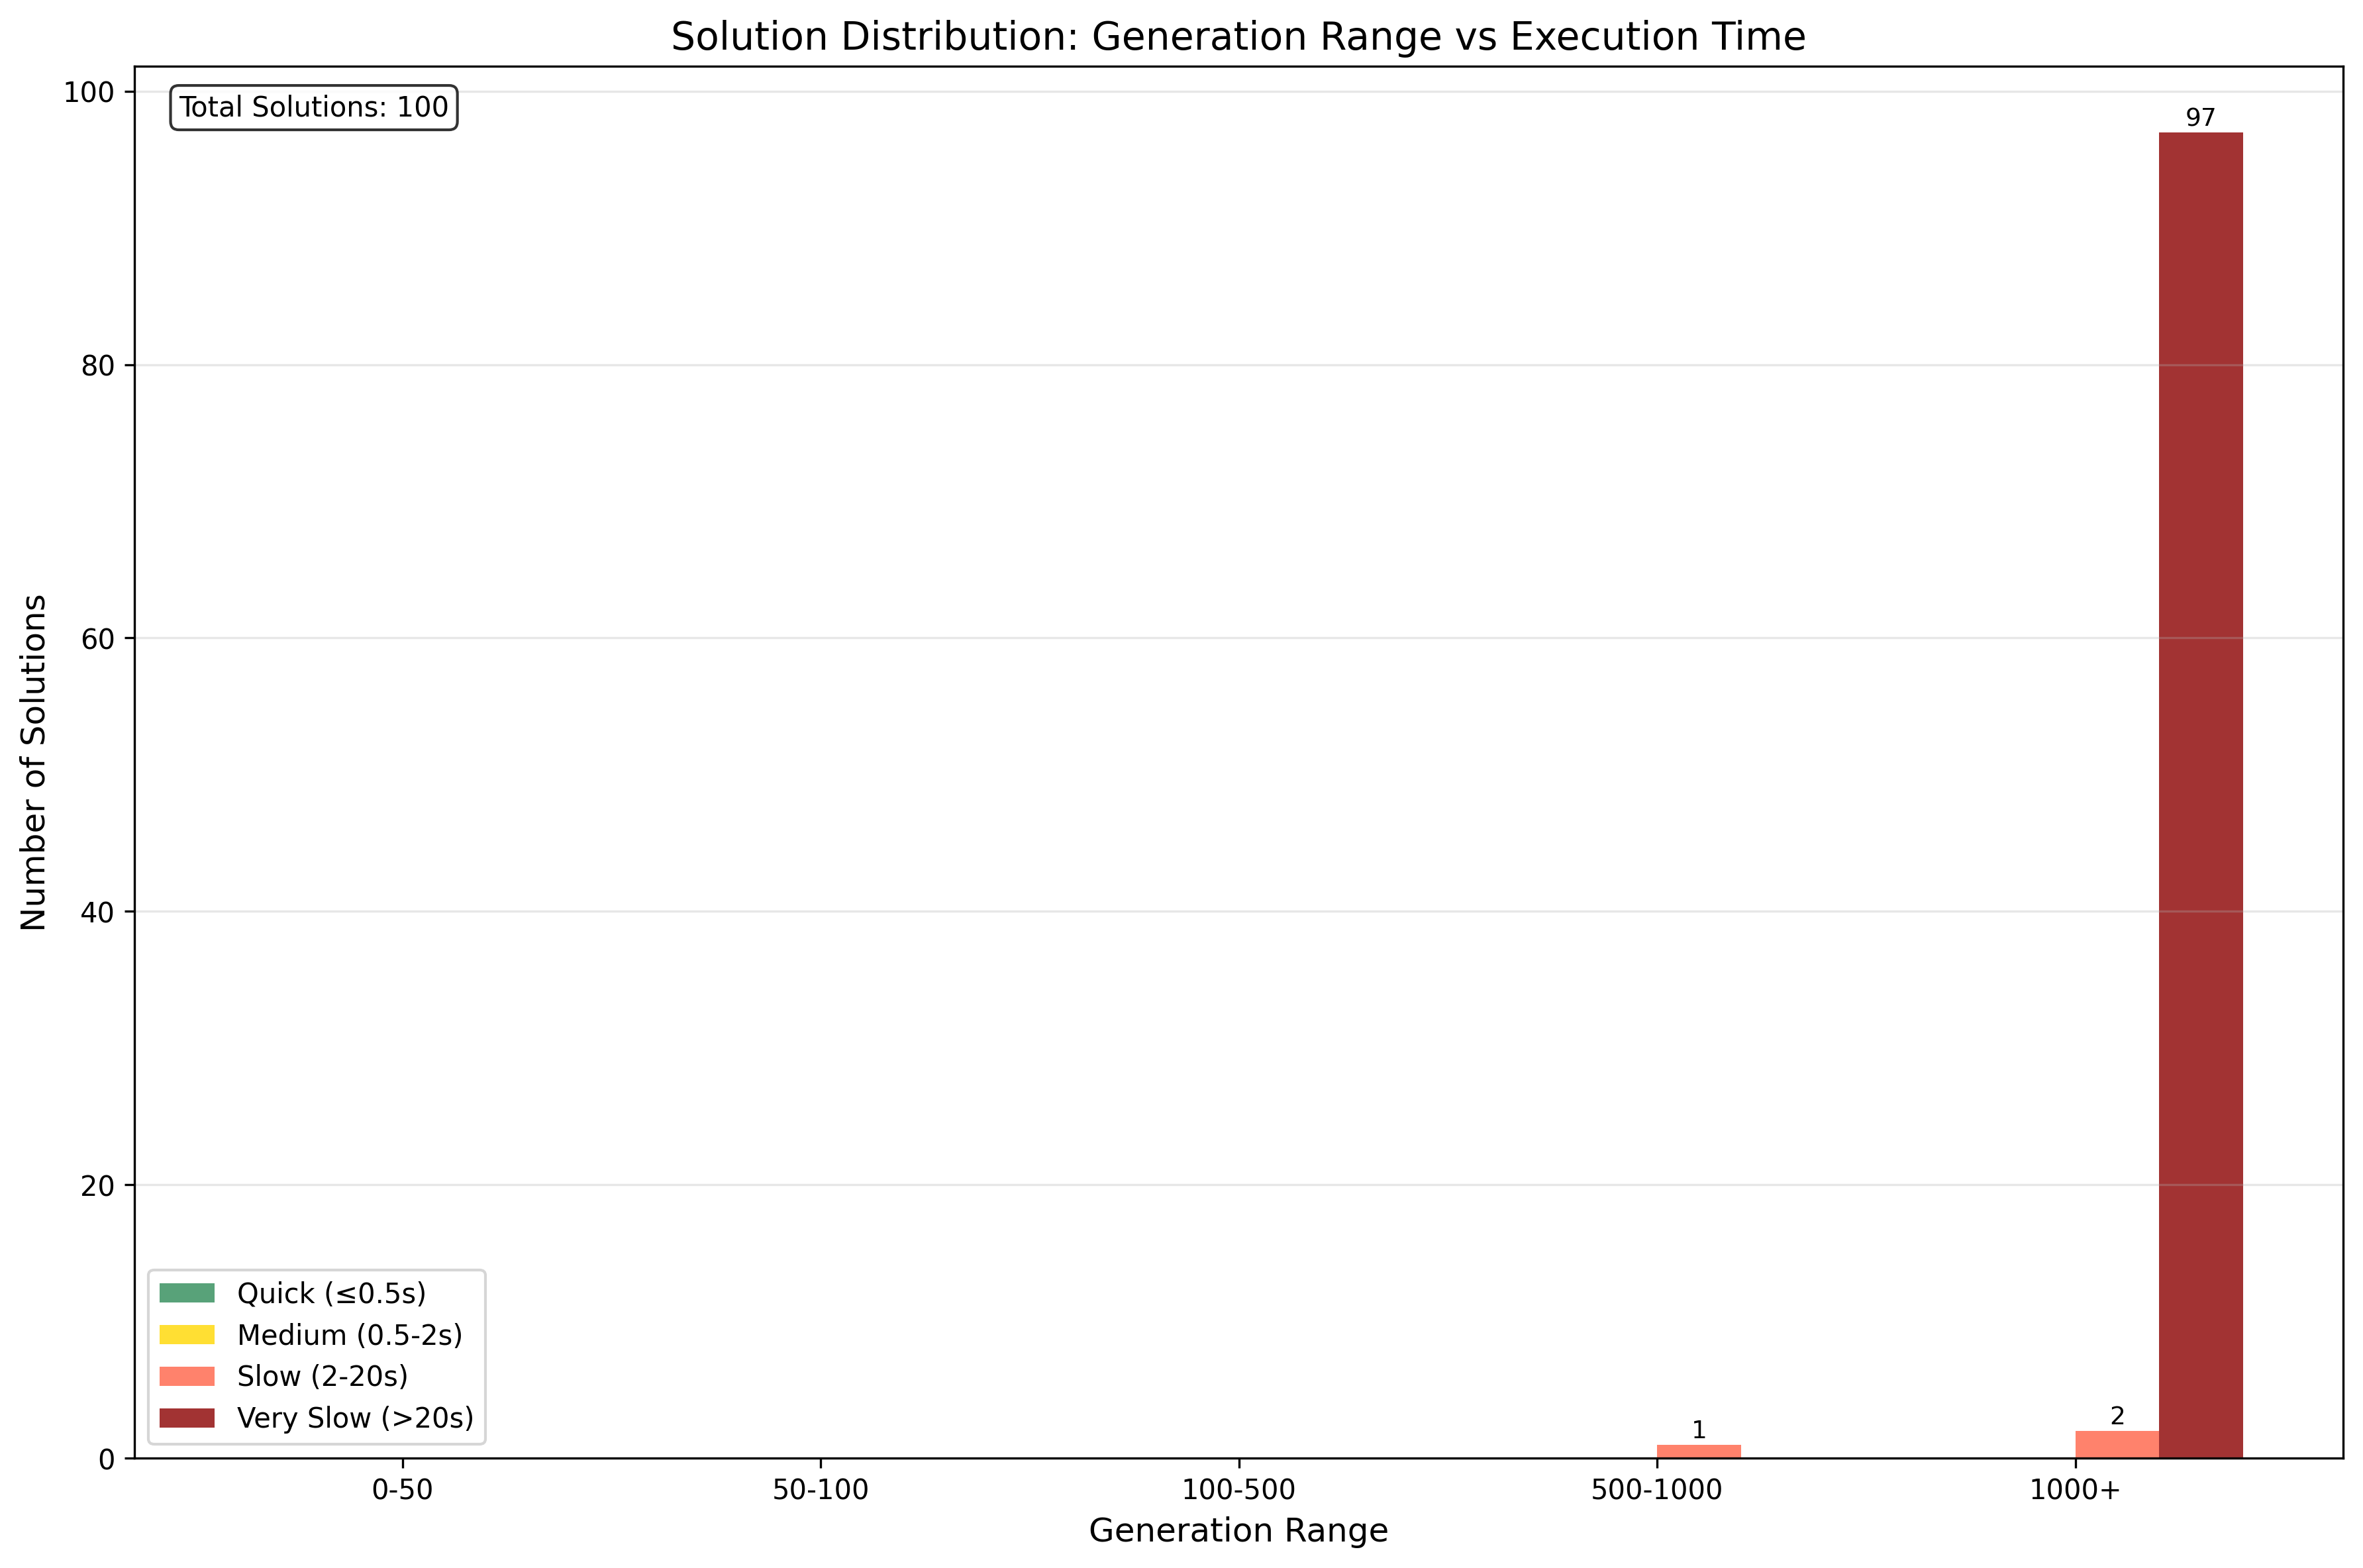
\includegraphics[width=0.8\textwidth]{resources/generation_execution_time_bars_hard.png}
\caption{Generation and execution time distribution for hard difficulty puzzles.}
\label{fig:generation_execution_time_bars_hard}
\end{figure}

\subsection{Test the performace by rule based algorithm}

We test the performace of the rule based algorithm with easy, medium and hard difficulty.

\begin{figure}[H]
\centering
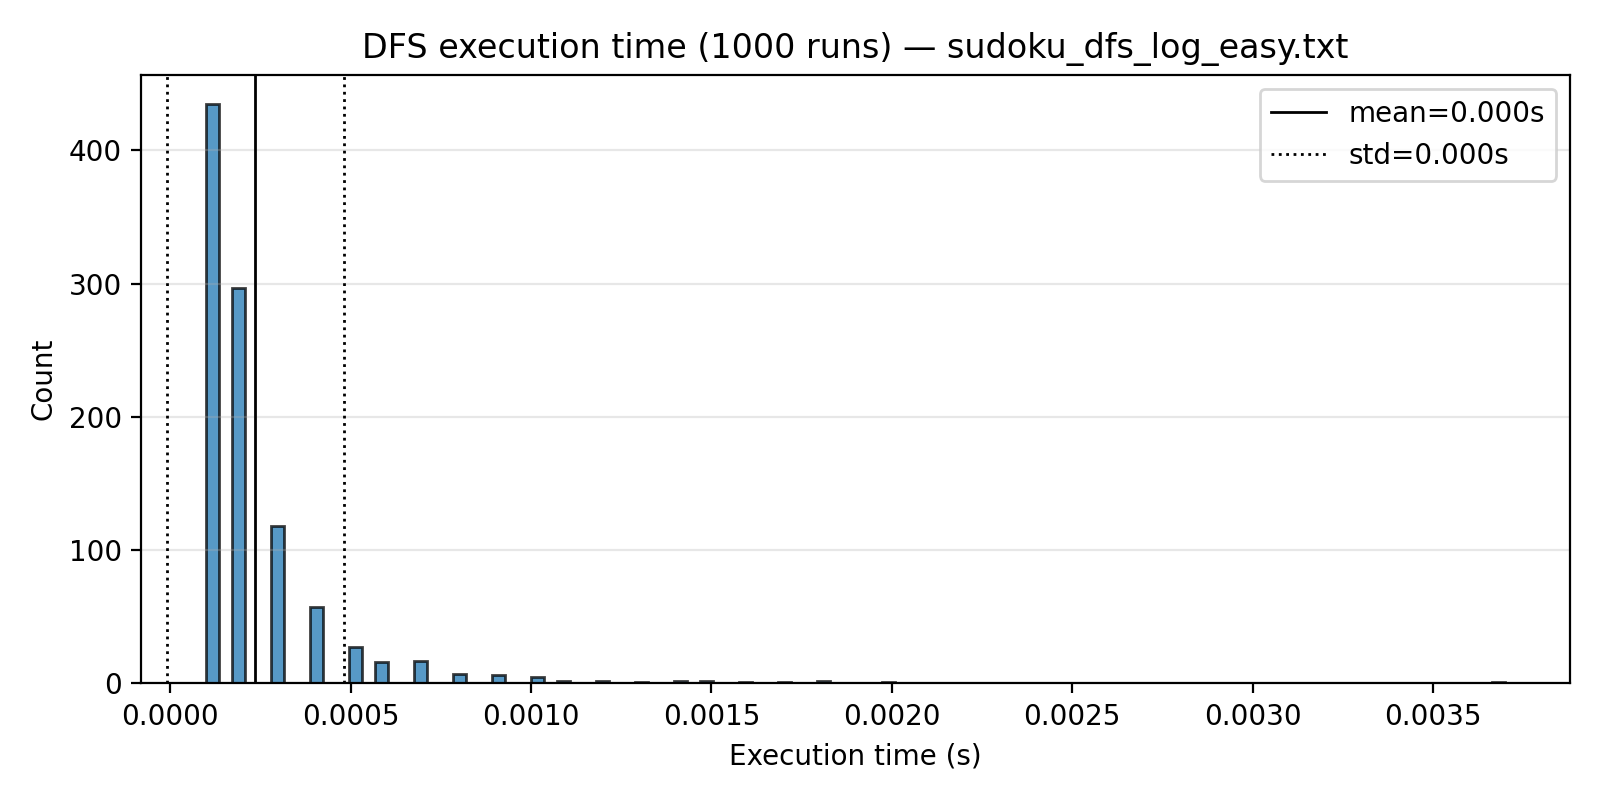
\includegraphics[width=0.8\textwidth]{resources/sudoku_dfs_log_easy_histogram.png}
\caption{sudoku\_dfs\_log\_easy\_histogram.}
\label{fig:sudoku_dfs_log_easy_histogram}
\end{figure}

\begin{figure}[H]
\centering
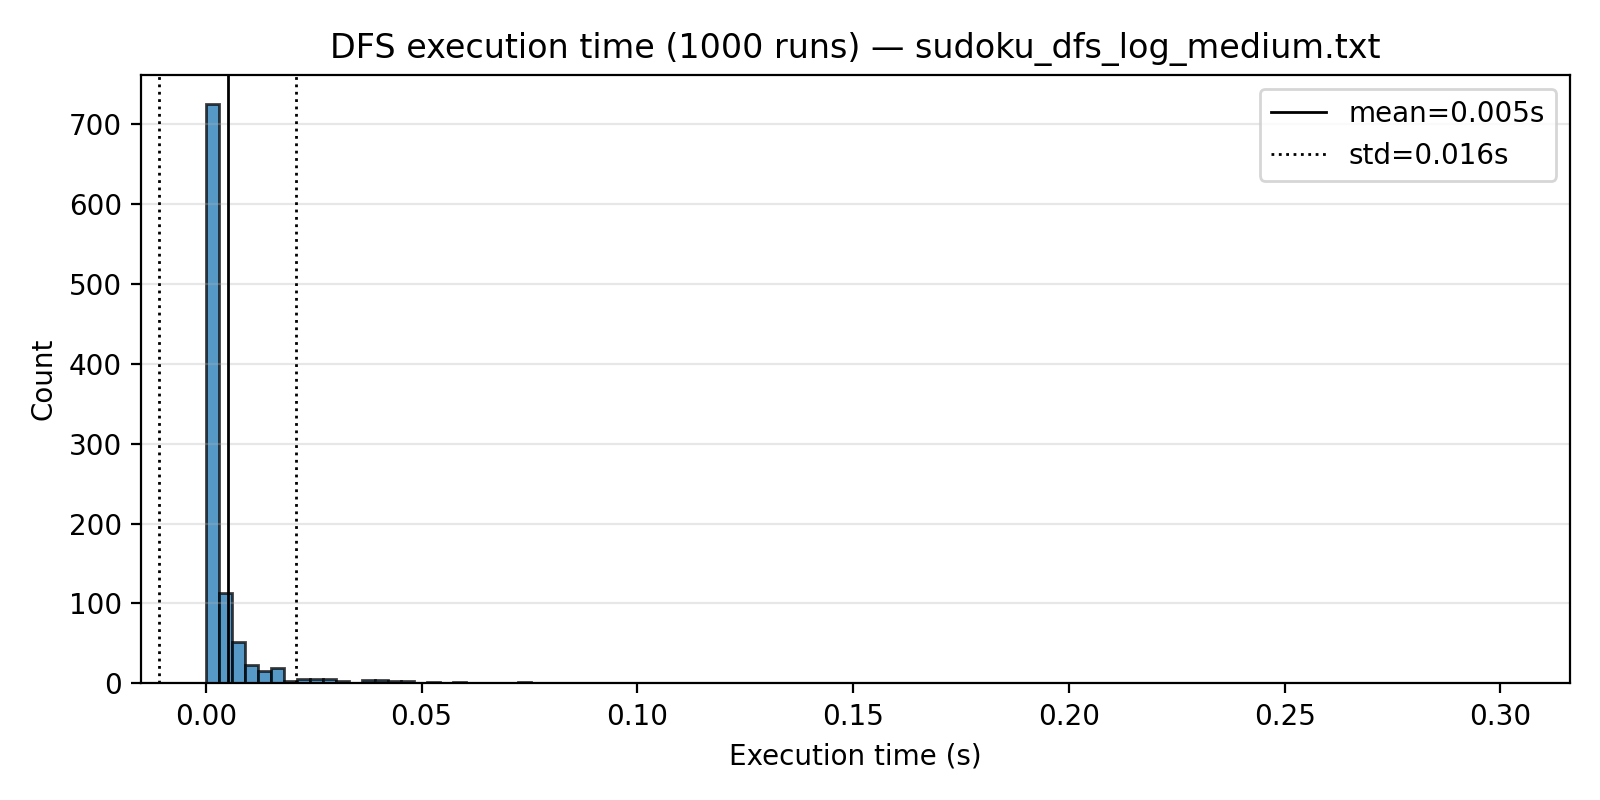
\includegraphics[width=0.8\textwidth]{resources/sudoku_dfs_log_medium_histogram.png}
\caption{sudoku\_dfs\_log\_medium\_histogram.}
\label{fig:sudoku_dfs_log_medium_histogram}
\end{figure}

\begin{figure}[H]
\centering
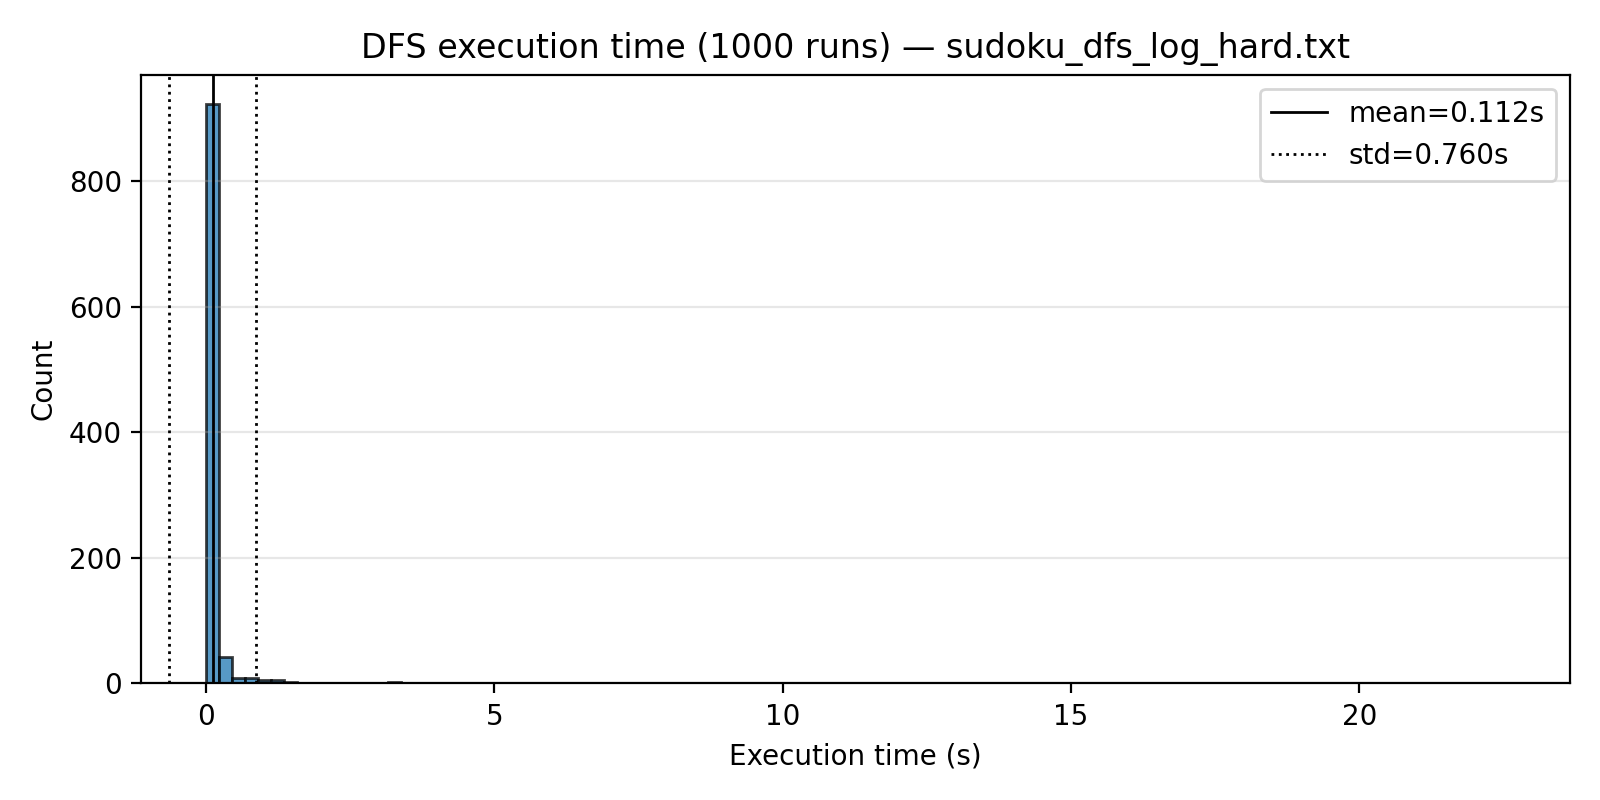
\includegraphics[width=0.8\textwidth]{resources/sudoku_dfs_log_hard_histogram.png}
\caption{sudoku\_dfs\_log\_hard\_histogram.}
\label{fig:sudoku_dfs_log_hard_histogram}
\end{figure}

The charts illustrate that no matter how hard the puzzle is, the rule based algorithm can solve it in a short time. Moreover, the execution time is very stable, only takes 0.001s-0.002s to solve each puzzle.
